
\documentclass[xcolor=dvipsnames]{beamer} % dvipsnames gives more built-in colors
\usepackage[utf8]{inputenc}
\usepackage[spanish]{babel}

\mode<presentation> {

\usetheme{CambridgeUS}

%\setbeamertemplate{footline} % To remove the footer line in all slides uncomment this line
\setbeamertemplate{footline}[page number] % To replace the footer line in all slides with a simple slide count uncomment this line

\setbeamertemplate{navigation symbols}{} % To remove the navigation symbols from

\definecolor{utfsmred}{HTML}{D60019}
\definecolor{utfsmyellow}{HTML}{F7AE00}
\definecolor{utfsmgreen}{HTML}{008452}
\definecolor{utfsmblue}{HTML}{004B85}


\newenvironment<>{rosa}[1][]{
  \setbeamercolor{block title example}{fg=white,bg=blue!75!black}%
  \begin{example}#2[#1]}{
  \end{example}
}



\usecolortheme[named=utfsmblue]{structure}
\setbeamercolor{titlelike}{parent=structure,fg=utfsmblue}
\setbeamercolor{frametitle}{fg=utfsmblue}

%\setbeamercolor{section in head/foot}{bg=Brown}
%\setbeamercolor{author in head/foot}{bg=Brown}
%\setbeamercolor{date in head/foot}{fg=Brown}

\setbeamercolor*{enumerate item}{fg=utfsmred}
\setbeamercolor*{enumerate subitem}{fg=utfsmred}
\setbeamercolor*{enumerate subsubitem}{fg=utfsmred}

\setbeamercolor*{itemize item}{fg=utfsmred}
\setbeamercolor*{itemize subitem}{fg=utfsmred}
\setbeamercolor*{itemize subsubitem}{fg=utfsmred}

\setbeamercolor{item projected}{bg=utfsmred}


\setbeamertemplate{itemize items}[square]
\setbeamertemplate{enumerate items}[default]


\setbeamercolor{section in head/foot}{bg=utfsmblue}

\setbeamercolor{block title}{bg=utfsmblue!80,fg=white}
\setbeamercolor{block title alerted}{bg=utfsmred!80,fg=white}
\setbeamercolor{block title example}{bg=utfsmgreen!80,fg=white}

\setbeamertemplate{sections/subsections in toc}[square]
\setbeamercolor{section number projected}{bg=utfsmblue,fg=white}


}


\usepackage{graphicx} % Allows including images
\usepackage{booktabs} % Allows the use of \toprule, \midrule and \bottomrule in tables
\usepackage{listings}
\lstset{ %
language=bash,
basicstyle=\normalsize\ttfamily,
keywordstyle=,
numbers=none,
numberstyle=\tiny\ttfamily,
stepnumber=1,
showspaces=false,
showstringspaces=false,
showtabs=false,
breaklines=true,
frame=tb,
framerule=0.5pt,
tabsize=4,
framexleftmargin=0.5em,
framexrightmargin=0.5em,
xleftmargin=0.5em,
xrightmargin=0.5em,
}

%----------------------------------------------------------------------------------------
%	TITLE PAGE
%----------------------------------------------------------------------------------------

\title{Trabajando con el filesystem}
\subtitle{\small{Seminario de Desarrollo de Software - Casa Central.}}
\author{Maximiliano Osorio\\\small{mosorio@inf.utfsm.cl}} 
\institute[UTFSM]
{
Universidad Técnica Federico Santa María
\medskip
}
\date{\today} % Date, can be changed to a custom date

\begin{document}

\maketitle
\begin{frame}{Comandos}
	\begin{figure}
		\centering
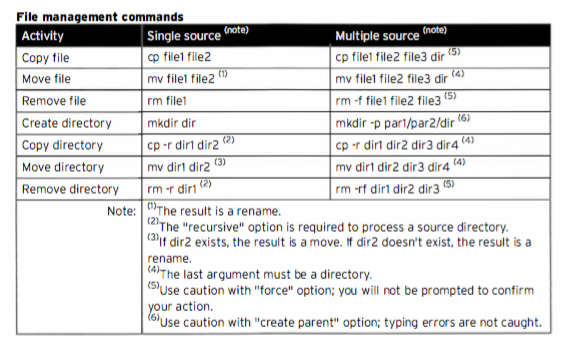
\includegraphics[width=\textwidth,height=0.8\textheight,keepaspectratio]{images/t1}	\end{figure}
\end{frame}



\begin{frame}[fragile]

    \frametitle{mkdir}
mkdir crea un directorio o subdirectorios.    
    \begin{lstlisting}
[mosorio@ssh ~]$ mkdir glob
    \end{lstlisting}
Si ruta completa no existe
	\begin{lstlisting}
[mosorio@ssh ~]$ mkdir super/tuper
mkdir: cannot create directory `super/tuper': No such file or directory
	\end{lstlisting}
	
Solución:
	\begin{lstlisting}
[mosorio@ssh ~]$ mkdir -p super/tuper

	\end{lstlisting}
\end{frame}


\begin{frame}[fragile]
    \frametitle{Ejemplo}
    
    \begin{lstlisting}
[mosorio@ssh ~]$ mkdir -p Videos/Watched
[mosorio@ssh ~]$ mkdir Documents
[mosorio@ssh ~]$ cd Documents
[mosorio@ssh Documents]$ mkdir ProyectX ProyectY
[mosorio@ssh Documents]$ mkdir -p Thesis/Chapter1 Thesis/Chapter2 Thesis/Chapter3
[mosorio@ssh Documents]$ cd
[mosorio@ssh ~]$ ls -R Videos/ Documents
...
    \end{lstlisting}
\end{frame}


\begin{frame}[fragile]
    \frametitle{Ejemplo}
    
    \begin{lstlisting}
[mosorio@ssh ~]$ cd Videos/
[mosorio@ssh Videos]$ touch v1.ogg
[mosorio@ssh Videos]$ cp v1.ogg v3.ogg
[mosorio@ssh Videos]$ ls
v1.ogg  v3.ogg  Watched
    \end{lstlisting}
\end{frame}



\begin{frame}[fragile]
    \frametitle{Ejemplo}
    
    \begin{lstlisting}
[mosorio@ssh Documents]$ touch thesis_c1.pdf thesis_c2.pdf
[mosorio@ssh Documents]$ cp thesis_c1.pdf thesis_c2.pdf Thesis/ ProyectX/
cp: omitting directory `Thesis/'
[mosorio@ssh Documents]$ ls -R 
...
[mosorio@ssh Documents]$ cp -r Thesis/ ProyectX
    \end{lstlisting}
\end{frame}


\begin{frame}[fragile]
    \frametitle{Ejemplo}
    
    \begin{lstlisting}
[mosorio@ssh Documents]$ mv ProyectX ProyectZ
[mosorio@ssh Documents]$ rm thesis_c2.pdf
[mosorio@ssh Documents]$ rm Thesis/
rm: cannot remove `Thesis/': Is a directory
[mosorio@ssh Documents]$ rm -r Thesis/
[mosorio@ssh Documents]$ rm -ri Proyect
ProyectY/ ProyectZ/
[mosorio@ssh Documents]$ rm -ri ProyectY/
rm: remove directory `ProyectY'? Y
    \end{lstlisting}
\end{frame}

\section{Ejercicio}

\begin{frame}[fragile]
    \frametitle{Brace expresion}
    
    \begin{lstlisting}
bash$ echo a{d,c,b}e
ade ace abe
    \end{lstlisting}
    \begin{lstlisting}
mkdir /usr/local/src/bash/{old,new,dist,bugs}
    \end{lstlisting}
\end{frame}

\begin{frame}{Expresiones regulares}
	\begin{figure}
		\centering

\includegraphics[width=\textwidth,height=0.8\textheight,keepaspectratio]{images/m1}	\end{figure}
\end{frame}


\begin{frame}[fragile]
    \frametitle{Preparando...}
    
    \begin{lstlisting}
[mosorio@ssh ~]$ mkdir glob
[mosorio@ssh ~]$ cd glob/
[mosorio@ssh glob]$ ls
[mosorio@ssh glob]$ touch alfa bravo charlie delta echo able baker cast dog easy
[mosorio@ssh glob]$ ls
able  alfa  baker  bravo  cast  charlie  delta  dog  easy  echo
    \end{lstlisting}
\end{frame}



\begin{frame}[fragile]
    \frametitle{Match file name using path name expansion}
    
    \begin{lstlisting}
[mosorio@ssh glob]$ ls *a*
able  alfa  baker  bravo  cast  charlie  delta  easy
[mosorio@ssh glob]$ ls [ac]*
able  alfa  cast  charlie
[mosorio@ssh glob]$ ls ????
able  alfa  cast  easy  echo
[mosorio@ssh glob]$ ls ?????
baker  bravo  delta
    \end{lstlisting}

\end{frame}


\begin{frame}[fragile]
    \frametitle{Match file name using path name expansion}
    
    \begin{lstlisting}
[mosorio@ssh glob]$ ls ~/glob/
able  alfa  baker  bravo  cast  charlie  delta  dog  easy  echo
[mosorio@ssh glob]$ echo ~/glob/
/home/mosorio/glob/
    \end{lstlisting}

\end{frame}


\begin{frame}[fragile]
    \frametitle{Match file name using path name expansion}
    \begin{lstlisting}
[mosorio@ssh glob]$ echo {Sunday,Monday,Tuesday,Wednesday}.log
Sunday.log Monday.log Tuesday.log Wednesday.log
[mosorio@ssh glob]$ echo file{1..3}.log
file1.log file2.log file3.log
[mosorio@ssh glob]$ echo file{a..c}.log
filea.log fileb.log filec.log
[mosorio@ssh glob]$ echo file{a,b}{1,2}.log
filea1.log filea2.log fileb1.log fileb2.log
[mosorio@ssh glob]$ echo file{a{1,2},b,c}.log
filea1.log filea2.log fileb.log filec.log
    \end{lstlisting}
\end{frame}

\begin{frame}{Preguntas}
	\begin{figure}
		\centering
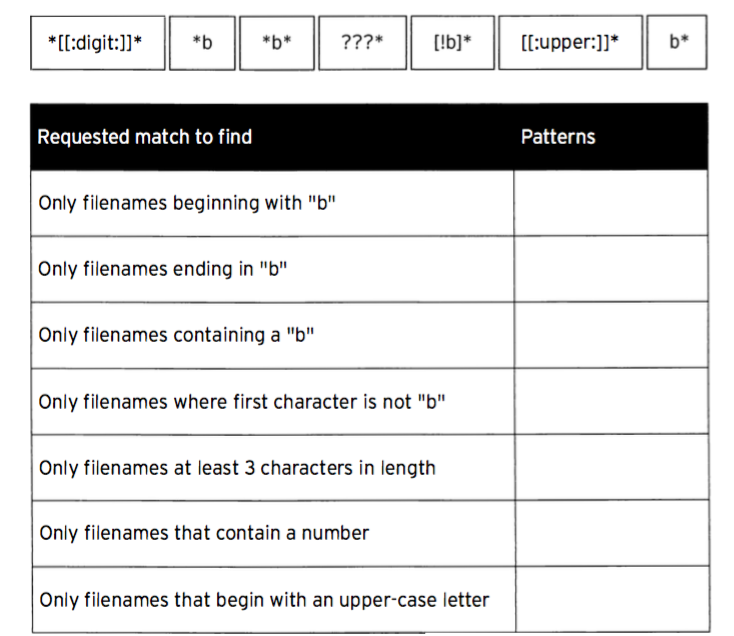
\includegraphics[width=\textwidth,height=0.8\textheight,keepaspectratio]{images/q1}	\end{figure}
\end{frame}
\begin{frame}{Respuestas}
	\begin{figure}
		\centering
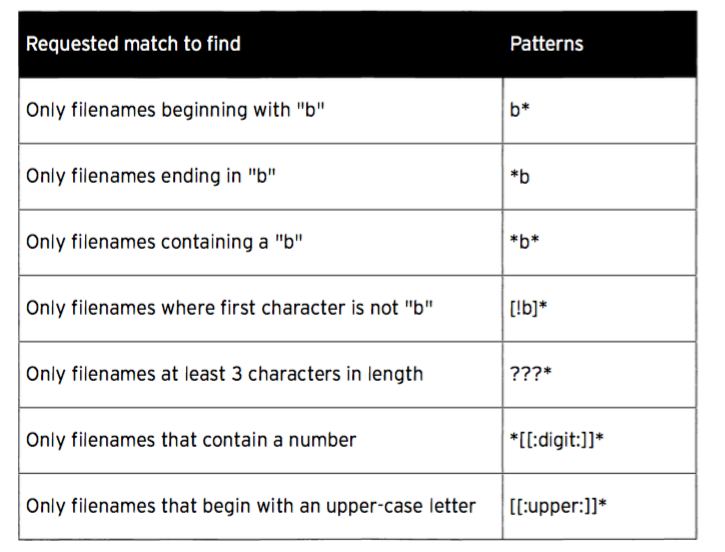
\includegraphics[width=\textwidth,height=0.8\textheight,keepaspectratio]{images/r1}	\end{figure}
\end{frame}



\begin{frame}[fragile]
    \frametitle{Subtitución de comandos}
 \begin{lstlisting}
`command`
$(command)
[mosorio@ssh glob]$ echo $(hostname)
ssh.inf.utfsm.cl
[mosorio@ssh glob]$ echo `hostname`
ssh.inf.utfsm.cl
    \end{lstlisting}
    
    \begin{block}{Consejo}
    Utilizar backticks no es recomendado dado que se puede confudir con las comillas simples y no puede colocar backticks dentro de backticks.
    	
    \end{block}
\end{frame}



\begin{frame}[fragile]

\begin{itemize}
	\item En bash shell hay caracteres reservados.
	\item Para escapar estos comandos se utiliza el backslash
	
\end{itemize}
    \frametitle{Subtitución de comandos}
    \begin{lstlisting}
[mosorio@ssh glob]$ host=$(hostname)
[mosorio@ssh glob]$ echo $host
ssh.inf.utfsm.cl
[mosorio@ssh glob]$ echo "$host"
ssh.inf.utfsm.cl
[mosorio@ssh glob]$ echo "\$host"
$host
    \end{lstlisting}
\end{frame}

\begin{frame}[fragile]
    \frametitle{Subtitución de comandos}
    \begin{lstlisting}
[mosorio@ssh glob]$ echo "La variable sera evaluada $(hostname)?"
La variable sera evaluada ssh.inf.utfsm.cl?
[mosorio@ssh glob]$ echo 'La variable sera evaluada $(hostname)?'
La variable sera evaluada $(hostname)?
    \end{lstlisting}
\end{frame}



\end{document}